\section{Anforderungen und Konzeption}
\subsection{Anforderungen}
Dieses Kapitel beschreibt die Anforderungen an das Projekt. Das Projekt ist die Implementierung und die Analyse einer Spiel-KI für das Spiel Ganz schön clever von Anfang bis Ende.
\subsubsection{Rahmenbedingungen}
Der zeitliche Rahmen der Arbeit beträgt vier Monate. In dieser Zeit ist zunächst ein Grundkonzept in Form eines Exposés vorzustellen. Anschließend soll dieses Konzept weiter verfeinert und validiert werden, was schließlich zur Vervollständigung des Projektes mit den gewünschten, sich aber zum Teil auch ändernden Anforderungen führen soll. 

Es ist eine Künstliche Intelligenz zu implementieren, welche das Spiel Ganz schön clever effizient spielen soll. Dazu muss zunächst die Spielumgebung entwickelt und implementiert werden. Mithilfe dieser soll ein Verfahren entwickelt werden, welches die Künstliche Intelligenz in dieser Umgebung trainieren soll.

Anschließend sind die Ergebnisse des Entwicklungsprozesses, sowie des Erzeugnisses selbst zu analysieren. Dies soll mithilfe geeigneter, schlüssiger sowie verständlicher Methoden und Visualisierungstechniken erfolgen.
\subsubsection{Das Spiel}
Das Spiel heißt Ganz schön clever. Es ist ein Würfelspiel bei dem es darum geht möglichst viele Punkte innerhalb einer vorgeschriebenen Rundenanzahl zu erreichen [siehe Grundlagen].

Zunächst soll ein Prototyp der Spielumgebung entwickelt werden, welcher später Stück für Stück erweitert werden soll, bis das Spiel mit allen Funktionalitäten implementiert worden ist.\\

Diese Funktionalitäten sind:

Die sechs farbigen Würfel, welche geworfen werden können und zufällig eine Würfelzahl von 1 bis 6 liefern. Es werden dabei immer alle aktuell gültigen Würfel gleichzeitig geworfen.

Einen Mechanismus, welcher die Würfel für die aktuelle Runde als ungültig markiert, sobald sie gewählt werden. Ungültige Würfel dürfen nicht gewählt werden [siehe Grundlagen].

Ein Mechanismus, welcher Würfel mit einer niedrigeren Augenzahl als der aktuell gewählte Würfel als ungültig für die Runde markiert, solange sich das Spiel nicht in einer Wahl vom Silbertablett oder einer Wahl mithilfe des Extra Wahl Boni befindet.

Ein Runden-System, bei dem insgesamt sechs Runden gespielt werden, in denen jeweils bis zu drei Würfe erfolgen, falls bei einem der Würfe noch gültige Würfel vorhanden sind. Zudem erfolgt nach jeder Runde die Auswahl eines Würfels vom Silbertablett, welches die ungültigen Würfel eines anderen Spielers beinhaltet. Wenn das Spiel alleine gespielt wird und es dadurch keinen anderen Spieler gibt, werden diese Würfel zufällig gewürfelt und dann drei davon auf das Silbertablett gelegt. Außerdem werden Boni am Anfang der ersten, zweiten, dritten und vierten Runde für alle Spieler freigeschaltet [siehe Grundlagen].

Die fünf farbigen Felder, gelb, blau, grün, orange und lila. Jedes Feld hat seine eigenen Regeln, wenn es darum geht wann ein Würfel gewählt werden darf, um eines der Kästchen auf diesem Feld auszufüllen [siehe Grundlagen]. Die Felder beinhalten verschiedene Boni, welche freigespielt werden, wenn bestimmte Kästchen oder Kombinationen aus diesen ausgefüllt worden sind [siehe Grundlagen].

Die sieben verschiedenen Boni, Fuchs, Extra Wahl, Neu Würfeln, Gelbes Kreuz, Blaues Kreuz, Grünes Kreuz, Orangene Vier, Orangene Fünf, Orangene Sechs sowie Lila Sechs [siehe Grundlagen]. Das beinhaltet sowohl das Erhalten, Speichern, sowie die Benutzung der Boni.

Ein Mechanismus, welcher Würfel, die mithilfe der Extra Wahl Boni gewählt worden sind, als ungültig markiert, damit diese nicht erneut in der selben Runde durch die Extra Wahl Boni gewählt werden können.

Ein Mechanismus, der Würfel zur richtigen Zeit wieder als gültig markiert. Dies erfolgt nach dem dritten Wurf in der Runde. Nach Extra Wahlen im eigenen Zug (nach dem dritten Wurf). Nach der Wahl vom Silbertablett des Gegners und nach Extra Wahlen, welche nach der Wahl vom Silbertablett des Gegners erfolgen.
\subsubsection{Die Künstliche Intelligenz}
Die Künstliche Intelligenz soll das Spiel möglichst Effizient spielen können. Es sollen geeignete Methoden zur Verfügung stehen, um die KI trainieren und mit ihr nach dem Training Vorhersagen treffen zu können. Außerdem sollte sie Möglichkeiten bieten verschiedene Parameter zu verändern, um den Trainingsprozess zu variieren und zu optimieren. 

Die wichtigsten dieser Parameter sind unter Anderem die Trainingsdauer, welche festlegt wie lange trainiert wird, Gamma, welches bestimmt wie zukunftsorientiert die KI ihre Entscheidungen fällt, die Größe und Art des neuronalen Netzen, das verwendet wird, welches bestimmt wie und präzise Merkmale von der Künstlichen Intelligenz erfasst werden können und mindestens einen Faktor, welcher das Ausmaß von Erkundung und Ausbeutung steuern soll. 

Außerdem soll die Implementierung auf einfache Art und Weise möglich sein, damit der vorhergesehenen zeitliche Rahmen der Arbeit eingehalten werden kann.
\subsection{Konzeption}
In diesem Kapitel wird das Grundkonzept der Künstlichen Intelligenz, sowie der Spielumgebung und deren Zusammenspiel beschrieben.

\begin{minipage}{\linewidth}
	Die Folgende Abbildung zeigt das Zusammenspiel von Spielumgebung und KI während des Trainingsprozesses:
	
	\vspace{0.5cm}
	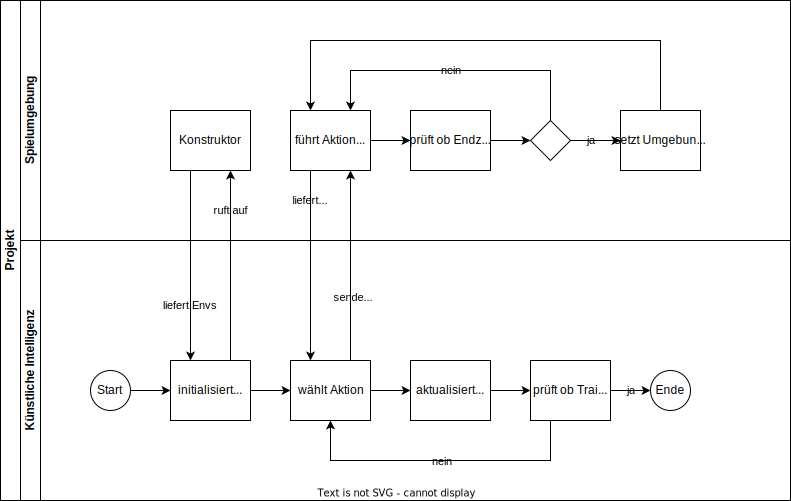
\includegraphics[width=1\textwidth]{Bilder/swimlane.drawio.pdf} 
	
	Abb. 6: Swimlane-Diagramm des Projektes \\

\end{minipage}

Der Trainingsprozess wird angestoßen, die Umgebung beziehungsweise die Umgebungen werden initialisiert. Dazu wird der Konstruktor der Umgebung aufgerufen. Daraufhin wird von der KI eine Aktion ausgewählt und an die Umgebung weitergeleitet. Die Umgebung führt diese Aktion aus und prüft ob der Endzustand des Spiels erreicht worden ist oder nicht. Wenn der Endzustand erreicht wurde, wird die Umgebung auf den Anfangszustand zurückgesetzt. Wenn der Endzustand nicht erreicht worden ist, wird der Prozess ohne Weiteres fortgesetzt. Daraufhin liefert die Umgebung der KI eine Belohnung für den ausgeführten Schritt und den neuen Zustand der Umgebung nach Ausführung der Schrittes/der Aktion.

Daraufhin aktualisiert die Künstliche Intelligenz ihr neuronales Netz mit der Policy und überprüft ob bereits genügend Zeit vergangen ist, um das Training zu beenden. Wenn die festgelegte Zeit vergangen ist wird das Training an dieser Stelle beendet. Wenn nicht wird die nächste Aktion gewählt und das Training wird fortgesetzt.

Dies ist lediglich eine vereinfachte Darstellung des Prozesses. In Wirklichkeit wird die Policy nicht nach jedem Schritt/jeder Aktion aktualisiert, sondern es wird erst eine festgelegte Menge an Aktions-Zustands-Paaren gesammelt. Dann wird das neuronale Netz mit dieser Gesamtmenge aktualisiert. Diese Aktions-Zustands-Paare ermöglichen es festzustellen welche Aktionen in welchen Zuständen zu einem guten Ergebnis geführt haben und welche nicht.
\subsubsection{Die Spielumgebung}
\begin{minipage}{\linewidth}
	Die folgenden beiden Abbildungen zeigen den prinzipiellen Funktionsablauf in der Spielumgebung. Dabei wird am Anfang eine Aktion entgegengenommen und am Schluss der neue Zustand dieser Umgebung nach Ausführung der Aktion zurückgegeben:\\
	
	\vspace{0.5cm}
	\includegraphics[width=1\textwidth]{Bilder/step3.drawio} 
	
	Abb. 7: Ablauf-Diagramm der Schritt Funktion 1 \\
\end{minipage}

Nachdem die Schritt Funktion angestoßen wird, werden die Variablen dieser Funktion zurückgesetzt, um einen klaren Schnitt zwischen vergangenen Aktionen und der aktuellen Aktion zu erzielen.

Anschließend wird die Aktion ihrem entsprechenden Ablauf zugeordnet. Es gibt Aktionen für Wahlen nach normalen Würfen, für Wahlen von Würfeln des Silbertablettes, sowie für das Nutzen von Boni. Außerdem gibt es eine Aktion, die nur dann wählbar ist, wenn keine der anderen Aktionen gewählt werden kann. Dies ist die Aktion für ungültige Züge.

Ist die Aktion nicht gültig, wird die Runde inkrementiert und der Zustand der Umgebung zurückgegeben.

Wird die Neu Würfeln Boni verwendet, werden die gültigen Würfel neu gewürfelt und anschließend der Zustand zurückgegeben.

Ist beides nicht der Fall kommt es zu einer Auswahl zwischen den wesentlichen Aktionen der Umgebung. Es gibt sogenannte Extra Wahlen, diese spalten sich auf in Extra Wahlen mit der Extra Wahl Boni und Wahlen vom Silbertablett des Mitspielers.

Handelt es sich nicht um eine Extra Wahl, so folgt eine Unterteilung in Extra Runden und Normale Runden. Bei Extra Runden wird eine der Boni verwendet, die es erlauben eines der farbigen Felder auszufüllen [siehe Grundlagen].

Handelt es sich nicht um eine Extrarunde muss es eine normale Wahl nach einem Standardwurf in einer der sechs Runden sein [siehe Grundlagen].

Handelt es sich um eine Extra Wahl mit Boni, dann steht noch die Aktion "aussetzen" zur Wahl. Diese inkrementiert lediglich die Runde, sodass das Spiel weiter fortgesetzt werden kann. Dies spiegelt die Möglichkeit im Spiel wieder auf die Nutzung der Extra Wahl Boni zu verzichten.\\

\begin{minipage}{\linewidth}

	\vspace{0.5cm}
	\includegraphics[width=1\textwidth]{Bilder/step2.drawio}
	
	Abb. 8: Ablauf-Diagramm der Schritt Funktion 2 \\
\end{minipage}

Der folgende Ablauf der Funktion gestaltet sich relativ ähnlich bei allen vier Varianten. Bei allen Vieren wird das Feld und das Kästchen ermittel, welches ausgefüllt werden soll und das entsprechende Kästchen wird anschließend ausgefüllt. Dann wird die Belohnung für diesen Schritt ermittelt.

Am Ende der Funktion unterscheiden sich die vier Varianten wieder. Bei der normalen Wahl nach einem Standardwurf werden die entsprechenden Würfel als ungültig markiert [siehe Grundlagen] und die Runde wird inkrementiert. Außerdem prüft die Funktion bei dieser Variante am Schluss ob das Spiel terminiert ist oder nicht.

Beim ausfüllen eines Feldes mittels Boni (keine Extra Wahl Boni) wird der entsprechende Boni dekrementiert.

Bei der Extra Wahl vom Silbertablett wird die Runde inkrementiert.

Bei der Extra Wahl mittels Boni wird der gewählte Würfel als ungültig markiert und der Extra Wahl Boni wird dekrementiert.

Bei allen vier Varianten wird am Ende der Funktion der aktuelle Zustand der Umgebung sowie die erhaltene Belohnung für den Schritt/die Aktion zurückgegeben.

\begin{minipage}{\linewidth}
	
\subsubsection{Die Künstliche Intelligenz}
Die folgende Abbildung zeigt die wesentlichen Hyperparameter, die bei der Entwicklung der Künstlichen Intelligenz von Bedeutung sind:\\

	\vspace{0.5cm}
	\includegraphics[width=1\textwidth]{Bilder/KI}
	
	Abb. 9: Hyperparameter der Künstlichen Intelligenz \\
\end{minipage}

Die Künstliche Intelligenz basiert auf der MaskablePPO Version von Stable Baselines 3 Contributing. Weiterhin sind Konfigurationen zu treffen, welche das Training beeinflussen und steuern. Diese Einstellungen nennt man Hyperparameter. Sie legen die Ausprägung gewisser Steuerelemente des MaskablePPO Algorithmus und ähnlicher Algorithmen fest.

Die wichtigsten Hyperparameter für das Projekt sind folgende:

Netzwerk Architektur: Die Netzwerk Architektur legt die Anzahl der Schichten und der Neuronen pro Schicht des Neuronale Netzes fest, welches für die Abbildung der Policy verwendet wird. Außerdem legt sie fest wie viele Neuronen es pro Schicht gibt [siehe Grundlagen]. Die Netzwerk Architektur ist so zu bestimmen, dass die Künstliche Intelligenz im Stande ist die Komplexität der Problemstellung mithilfe dieser zu erfassen und gleichzeitig zu gewährleisten, dass die Trainingsdauer, die Systemauslastung dadurch nicht zu hoch steigen und es möglichst keine Überanpassung an die Trainingsdaten gibt. Da es sich bei dem Neuronalen Netz um ein Multilayer Perceptron handelt, sind alle Neuronen einer Schicht mit allen der vorherigen und folgenden Schicht verbunden [siehe Grundlagen]. Dies führt dazu, dass die Rechenleistung für das Updaten der Gewichte der Policy exponentiell steigt, je komplexer das Neuronale Netz wird. Dies führt zu einer gesteigerten Trainingsdauer und Systemauslastung. Außerdem tendieren zu komplexe Neuronale Netze dazu sich stark an die Trainingsdaten anzupassen, was zu Überanpassung führen kann. Zu komplexe Netze generalisieren tendenziell schlechter auf neue Datensätze, die sich stark von der Trainingsdaten unterscheiden.

Anzahl der Umgebungen: Eine erhöhte Anzahl an Trainingsumgebungen ermöglicht es vor allem bei Nutzung von CUDA (GPU) parallel Daten aus mehreren Umgebungen zu sammeln und zu verarbeiten. Dies erhöht die Trainingsgeschwindigkeit, da ein erheblicher Teil der Trainingsdauer in diesem Projekt davon abhängt, wie schnell die nötigen Trainingsdaten aus den Umgebungen generiert werden können. Außerdem erhöht die Nutzung von CUDA die Geschwindigkeit von Policy Updates enorm, da viele der Berechnungen im Neuronalen Netz somit parallel abgearbeitet werden können. Allerdings erhöht die Anzahl der Umgebungen die RAM Auslastung enorm und die CPU Auslastung mittelmäßig stark, was dazu führt, dass es ineffizient wäre auf dem verwendeten System (Nvidia Geforce GTX 1070, Intel i5 8600k, 16GB RAM) deutlich mehr als 32 Umgebungen laufen zu lassen.

Aktivierungsfunktion: Die Aktivierungsfunktion legt fest, wann und wie stark Neuronen ihre Signale an die folgenden Neuronen weiterleiten. Im Projekt wird vor allem die ReLU Funktion verwendet, da diese standardmäßig vom Algorithmus verwendet wird und im allgemeinen sowie spezifisch in diesem Projekt gute Ergebnisse zu erzielen scheint. Die Formel der ReLU Funktion lautet: f(x) = max(0,x). Die ReLU Funktion gibt, wenn der Wert kleiner Null ist Null zurück und ansonsten den Wert selbst. Die folgende Abbildung zeigt den Graphen der ReLU Funktion:\\

\begin{minipage}{\linewidth}
	\vspace{0.5cm}
	\includegraphics[width=1\textwidth]{Bilder/ReLU.png}
	
	Abb. 10: ReLU Funktion \\
\end{minipage}

Gamma: Gamma legt fest wie stark Zukünftige Belohnungen wertgeschätzt werden. Es fungiert als eine Art Multiplikator. Potenzielle Belohnungen werden pro Spielschritt, den sie in der Zukunft entfernt liegen würden, mit Gamma multipliziert. Gamma ist so zu wählen, dass das Modell lernt, die bestmöglichen Aktionen zu wählen, um insgesamt das beste Ergebnis zu erzielen. Zu hohe Werte von Gamma können dazu führen, dass kurzzeitige Belohnungen vernachlässigt werden, was zu einem schlechteren Gesamtergebnis führen kann, wenn diese von besonderer Bedeutung sind. Zu niedrige Werte von Gamma können wiederum dazu führen, dass der Agent nicht zukunftsorientiert handelt und somit kein gutes Gesamtergebnis erzielt, da er sich nur auf kurzfristige Belohnungen konzentriert, anstatt in die Zukunft zu schauen und dieser Wert zuzumessen. In diesem Projekt bewegt sich der Wert von Gamma im Allgemeinen in einem Bereich zwischen 0.5 und 1.

Die Lernrate: Die Lernrate bestimmt wie stark Updates des Neuronalen Netzes und seiner Gewichtungen pro Updateschritt ausfallen. Zu große Werte für die Lernrate können zu einem instabilen Training führen, da die Updates somit stark vom gewählten Trainingsdatensatz abhängen. Zu niedrige Werte führen wiederum zu einer Erhöhung der nötigen Trainingsdaten und Trainingsdauer. Der Wert für die Lernrate bewegt sich im Projekt üblicherweise zwischen Werten von 0.0003 bis zu 0.0003x32.

Entropie Koeffizient: Der Entropie Koeffizient bestimmt das Maß an Exploration des Modells. Je höher der Entropie Koeffizient ist desto stärker Belohnt das Modell neue beziehungsweise bisher wenig erkundete Aktionen oder Zustände. Ein zu hoher Wert führt dazu, dass das Modell nicht lernt bereits funktionierende Taktiken genügend zu verfestigen. Ein zu niedriger Wert führt dazu, dass das Modell sich relativ schnell auf eine bisher vergleichsweise gut funktionierende Strategie festlegt und diese verfestigt. Der Entropie Koeffizient bewegt sich innerhalb des Projektes meist zwischen Werten von 0.05 und 0.3, wobei sich ein Wert um die 0.1 als stabil und effizient herausgestellt hat.

Clip Range: Die Clip Range ist spezifisch für den PPO Algorithmus. Sie legt fest wie stark Policy Updates sein dürfen und ab welchem Schwellwert die Updates abgeschnitten werden. Mit Abschneiden ist gemeint, dass die Updates zwar noch durchgeführt werden, allerdings darf die Policy nach dem Update nur maximal um einen bestimmten Wert von der vorherigen abweichen. Die standardmäßige Clip Range beläuft sich auf 0.2. Innerhalb des Projektes werden auch andere Werte getestet.

nSteps: nSteps legt fest, wie viele Aktions-Zustands-Paare gesammelt werden bevor ein Update des Neuronales Netzes erfolgt.

nEpochs: nEpochs legt fest wie oft das selbe Datenpaket von nSteps für das Training benutzt wird bevor es verworfen wird. Je öfter man es verwendet desto weniger Daten braucht man und desto schneller verläuft das Training. Allerdings sollte der selbe Datensatz nicht zu häufig verwendet werden, um Überanpassung zu vermeiden. nEpochs beträgt im Rahmen des Projektes üblicherweise einen Wert zwischen 5 und 11.

Batch Size: Das Datenpaket von nSteps wird vor der Verwendung für das Updaten des Neuronalen Netzes in kleinere Datenpakete, die sogenannten Batches, zerlegt. Daraufhin werden Updates mit jedem dieser Batches durchgeführt. Die Aufteilung erfolgt per Zufall, daher ist mit hoher Wahrscheinlichkeit keines der Datenpakete (Batches) wie das andere, selbst wenn das selbe Gesamtdatenpaket durch ein hohes nEpochs viele male verwendet wird. Batch Size legt fest wie groß diese kleineren Datenpakete (Batches) sind.

Die Trainingsdauer: Die Trainingsdauer legt fest wie lange trainiert wird. Die Implementierung von Stable Baselines verwendet standardmäßig Timesteps zur Messung von Zeit. Eine Timestep ist ein ausgeführter Schritt beziehungsweise eine ausgeführte Aktion in einer Umgebung. Die Timesteps von mehreren parallel laufenden Umgebungen werden aufsummiert, somit kommt es nicht zu vermehrtem Training nur durch Erhöhung der Umgebungsanzahl bei gleichbleibender Trainingsdauer in Timesteps.
\subsubsection{Einschränkungen}
Aus zeitlichen Gründen ergeben sich einige Einschränkungen für das Design der Implementierung. Das Spiel endet nach der Wahl des Würfels nach dem dritten Wurf in der sechsten Runde. Somit kann die Extra Wahl Boni kein letztes mal benutzt werden und es gibt in der letzten Runde auch keine Wahl vom Silbertablett. Außerdem werden beim solo Spiel nicht die niedrigsten sechs Würfel des Wurfes auf das Silbertablett des viruellen Mitspielers gelegt, sondern drei zufällige.

Des weiteren ist ChatGPT nicht zur Codegenerierung über den Prototypen hinaus zu nutzen. Der Code soll nach Erstellung der Prototypen selbstständig geschrieben werden. Auch soll ChatGPT nicht genutzt werden um Text für die Bachelorarbeit selbst zu generieren.